%\usepackage{float}
\chapter[Introdução]{Introdução}

O projeto que será descrito neste relatório é referente a um robô semi-automático de limpeza, nomeado como “Quirby”. Para o seu desenvolvimento, serão integradas diversas áreas da engenharia, tais como a engenharia eletrônica (responsável pela seleção dos componentes eletrônicos e conexão dos mesmos aos elementos de estrutura), a engenharia de software (responsável pelo desenvolvimento de algoritmos para realizar o controle do robô, além do desenvolvimento de um aplicativo para ampliar as funções do “Quirby”), a engenharia de energia (responsável por realizar o dimensionamento de baterias para garantir uma autonomia satisfatória ao eletrodoméstico), além das engenharias aeroespacial e automotiva (que atuam na escolha de materiais e projeção das peças estruturais do robô de limpeza).
O “Quirby” visa auxiliar na resolução um problema muito comum para grande parte das pessoas atualmente: manter a casa limpa. Para automatizar um serviço doméstico, é empregado o uso de um robô aspirador, que mantém o chão da casa sem poeira, e que necessita de pouca intervenção humana, tendo em vista que o mesmo é um projeto semi-autônomo.


\section{Detalhamento do Problema}

O projeto “Quirby” surge para facilitar uma atividade doméstica que necessita ser realizada de forma constante para a manutenção de um ambiente limpo. Por ser um produto semi-autônomo, o Quirby possibilita a redução do tempo gasto com a limpeza de ambientes domésticos, e sua ativação por intermédio de um aplicativo \textit{mobile} o torna ainda mais prático e acessível para diversos perfis de usuário.

\section{Levantamento de Normas Técnicas Relacionadas ao Problema}
Para o desenvolvimento do presente projeto, são necessárias as leituras de algumas normas técnicas de extrema relevância para o escopo que irá ser explorado ao longo do projeto. Elas estão relacionadas ao desenvolvimento de máquinas e equipamentos eletrodomésticos, e visam garantir a segurança dos usuários.

Para isso, há a NR12 \cite{NR12}, utilizada em relação ao maquinário usado na criação do nosso projeto. Além disso, para o uso do aplicativo mobile tem-se a Lei Geral de Proteção de Dados Pessoais \cite{lgpd}, para proteger o cliente.

Também há a ISO 9283 \cite{iso9283} que visa facilitar o entendimento entre usuários e fabricantes de robôs e sistemas robóticos. Define as principais características de funcionamento e descreve como devem ser especificados. Recomenda-se realizar 14 testes para verificar se o robô obedece à especificação. A norma brasileira ABNT NBR 60335-1:2010 trata da segurança de aparelhos eletrodomésticos e similares, cuja tensão nominal não seja superior a 250 V, para aparelhos monofásicos, e 480 V para outros aparelhos.

\section{Identificação de Soluções Comerciais}

\begin{table}[H]
\centering
\caption{\label{solComerciais} Concorrentes no mercado}
\begin{tabular}{llll}
                                                                     & \cellcolor[HTML]{D9D9D9}\textbf{Multilaser HO041}                          & \cellcolor[HTML]{D9D9D9}\textbf{Roomba 614 iRobot}                                 & \cellcolor[HTML]{D9D9D9}\textbf{Robô Aspirador Midea}                                                                                                        \\
\rowcolor[HTML]{DBEEF3} 
\textbf{\begin{tabular}[c]{@{}l@{}}Custo \\ aproximado\end{tabular}} & R\$350,00                                                                  & R\$1833,49                                                                         & R\$3600,00                                                                                                                                                   \\
\rowcolor[HTML]{DBEEF3} 
\textbf{Eficiência}                                                  & \begin{tabular}[c]{@{}l@{}}Média, \\ apenas modo \\ aleatório\end{tabular} & \begin{tabular}[c]{@{}l@{}}Superior ao Multilaser, \\ mais popular hoje\end{tabular} & \begin{tabular}[c]{@{}l@{}}Superior aos demais, \\ é automático e \\ realiza o mapeamento do \\ ambiente, atuando de \\ maneira mais eficiente.\end{tabular} \\
\rowcolor[HTML]{DBEEF3} 
\textbf{Autonomia}                                                   & 2 horas                                                                    & 1 hora                                                                          & 3 horas                                                                                                                                                      \\
\rowcolor[HTML]{DBEEF3} 
\textbf{Conectividade}                                               & Não há.                                                                    & Conexão com app.                                                                   & Conexão com app.                                                                                                                                            
\end{tabular}
\end{table}

\section{Objetivo Geral do Projeto}
O objetivo geral do projeto consiste em desenvolver um protótipo de produto similar aos indicados na tabela \ref{solComerciais}.

\section{Objetivos Específicos do Projeto}

 Criar um dispositivo que consiga limpar um determinado ambiente em tempo hábil, dentro de sua autonomia de bateria, que deve atender os requisitos mínimos dispostos neste documento. Além de manter conectividade estável entre o robô, o servidor e o aplicativo, fazer um design relativamente compacto, que seja hábil para acessar locais de difícil acesso, como embaixo dos móveis.

\subsection{Metodologia}
	Para definir os objetivos do projeto Quirby e auxiliar no levantamento de requisitos, a equipe utilizou a metodologia Lean Inception. O Lean Inception é uma forma de workshop e brainstorming colaborativo dividido em várias etapas e atividades que direcionam a equipe na construção do produto, auxiliando na definição do Produto Mínimo Viável \cite{caroli}.
	Utilizando esta metodologia, definiu-se a Visão do Produto, Lista É/Não É - Faz/Não Faz, Objetivos do Produto e do Negócio, Personas, Jornada do Usuário, Brainstorming de Funcionalidades, Revisão Técnica, de Negócio e de Usuário e o Sequenciador de Funcionalidades.
 \subsubsection{Visão do Produto}
 De forma colaborativa, a equipe discutiu a Visão do Produto, em especial seu público alvo, funções principais, nome e diferenciais \cite{caroli}. A visão da equipe pode ser vista no anexo, através da figura \ref{visao do produto}.

 \subsubsection{Lista É/Não É - Faz/Não Faz}
 Apresenta as noções e concepções básicas acerca do que o produto é e não é, assim como do que faz e não faz. Para facilitar o levantamento e entendimento de seus objetivos e escopo \cite{caroli}. Os conceitos aplicados no Quirby podem são vistos no anexo, a partir da figura \ref{lista e nao e}.

 \subsubsection{Objetivos do Produto e do Negócio}
 Durante esta atividade, os participantes compartilharam seu entendimento do projeto para chegar a um consenso acerca dos pontos principais do produto e do negócio, para auxiliar no levantamento e esclarecimento dos objetivos \cite{caroli}. Portanto, para resumir o entendimento coletivo acerca do projeto, tem-se a figura \ref{objetivos produto}.
 
 \subsubsection{Personas}
 De acordo com \cite{caroli} “Uma persona cria uma representação realista de usuários, auxiliando o time a descrever funcionalidades do ponto de vista de quem vai interagir com o produto final.” Ao considerar os usuários finais do produto e seus objetivos, a equipe elaborou personas e uma anti persona que podem ser vistas no anexo, pela figura \ref{Personas}.

 \subsubsection{Jornada do Usuário}
 A Jornada do Usuário busca caracterizar a interação do usuário com o produto, descrevendo o percurso de um usuário por uma sequência de passos, que representam diferentes pontos de contato com o produto, para alcançar seus objetivos \cite{caroli}. Este conceito, aplicado ao robô, pode ser visualizado na figura \ref{Jornada do Usuário}, no qual descreve a jornada do usuário com o produto, passo a passo.
 
\subsubsection{Brainstorming de funcionalidades}
De forma colaborativa, realizou-se um Brainstorming de possíveis ações e interações do usuário com o produto \cite{caroli}.  Os resultados desta ação colaborativa são vistos na figura \ref{Brainstorming}.

\begin{figure}[H]
\centering
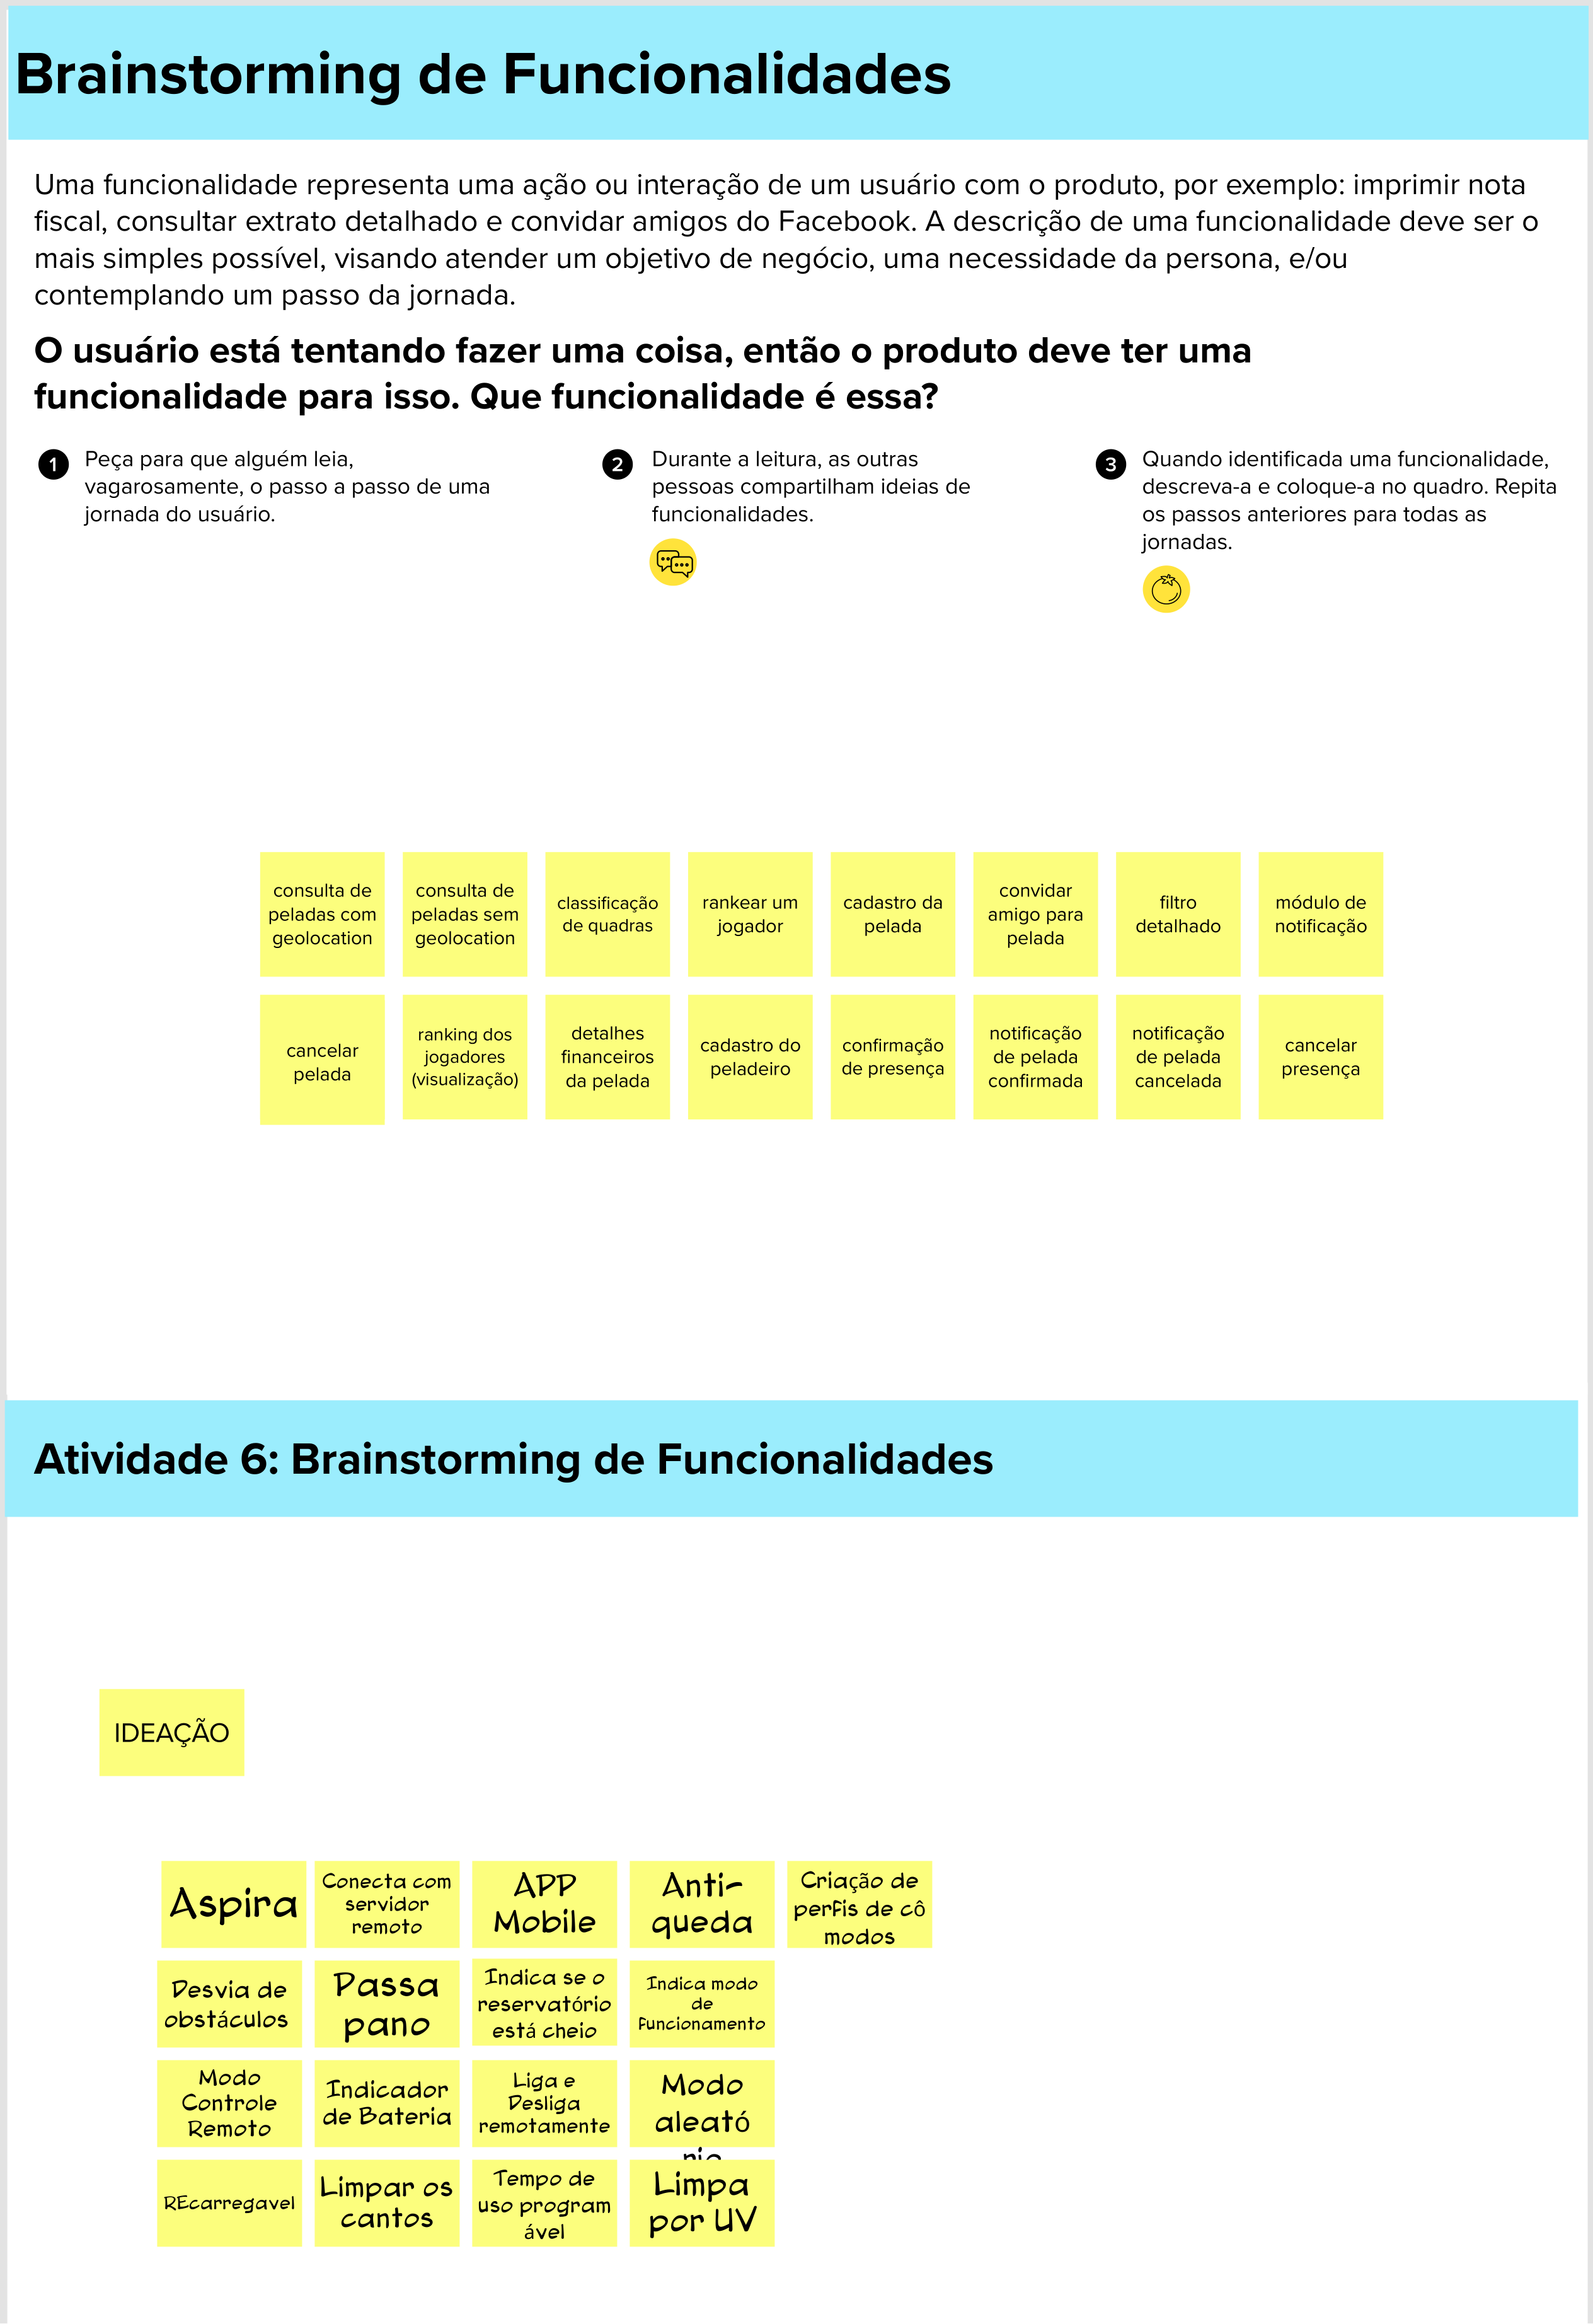
\includegraphics[height=0.7\textheight]{figuras/Lean Inception/Mural - Brainstorm.png}
\caption{Brainstorming \\ Fonte: Autoria própria, 2023.}

\label{Brainstorming}
\end{figure}
 

\subsubsection{Revisão Técnica, de Negócio e de Usuário}
Segundo Caroli (2018), esta revisão tem o objetivo de discutir como a equipe compreende o valor técnico, o de negócio e o de usuário para cada funcionalidade. Portanto, o grupo dividiu as funcionalidades para atender o conceito da revisão técnica e pode ser observado pela figura \ref{revisao}.

\begin{figure}[H]
\centering
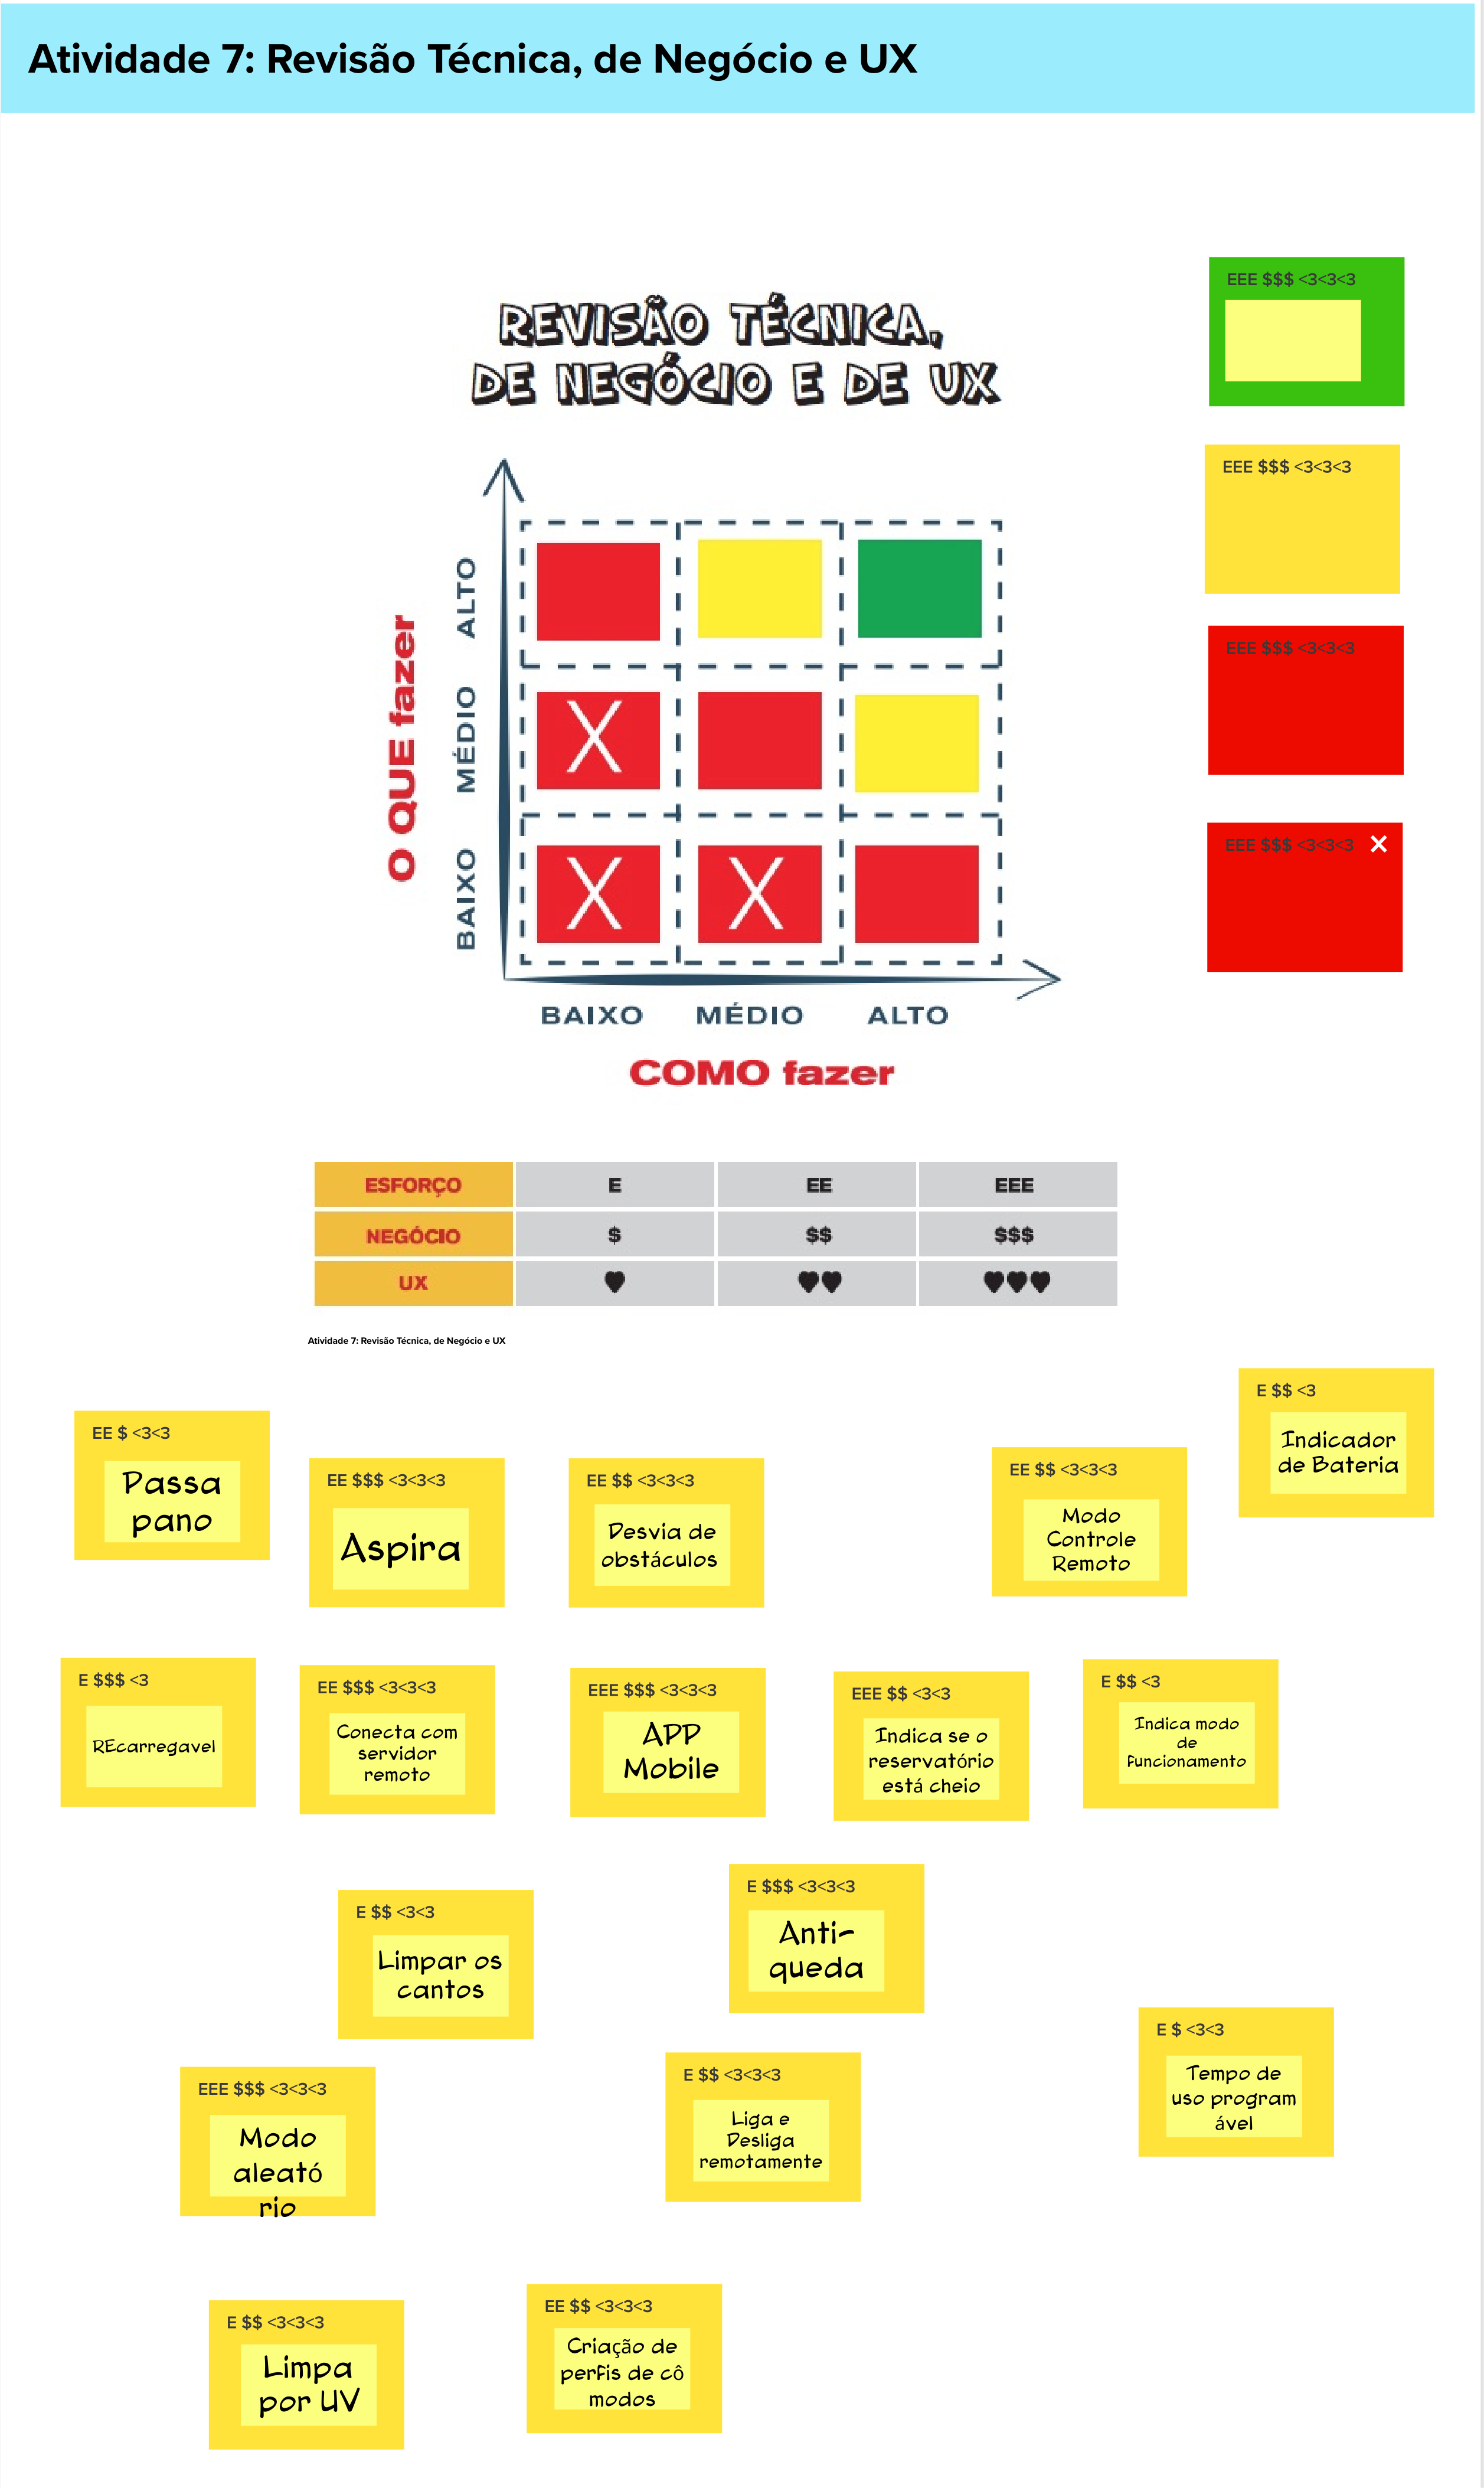
\includegraphics[height=0.7\textheight]{figuras/Lean Inception/Mural - Revisão Técnica, de Negócio e de UX.png}
\caption{Revisão Técnica, de Negócio e de Usuário \\ Fonte: Autoria própria, 2023.}
\label{revisao}
\end{figure}
 

\subsubsection{Sequenciador de Funcionalidades}
O Sequenciador de funcionalidades foi utilizado para organização e visualização das funcionalidades e da sequência de validação incremental do produto \cite{caroli}. Desta forma, utilizou-se o sequenciador para a melhor visualização do produto e suas funcionalidades, como pode ser visto na figura \ref{sequenciador}.

\begin{figure}[H]
\centering
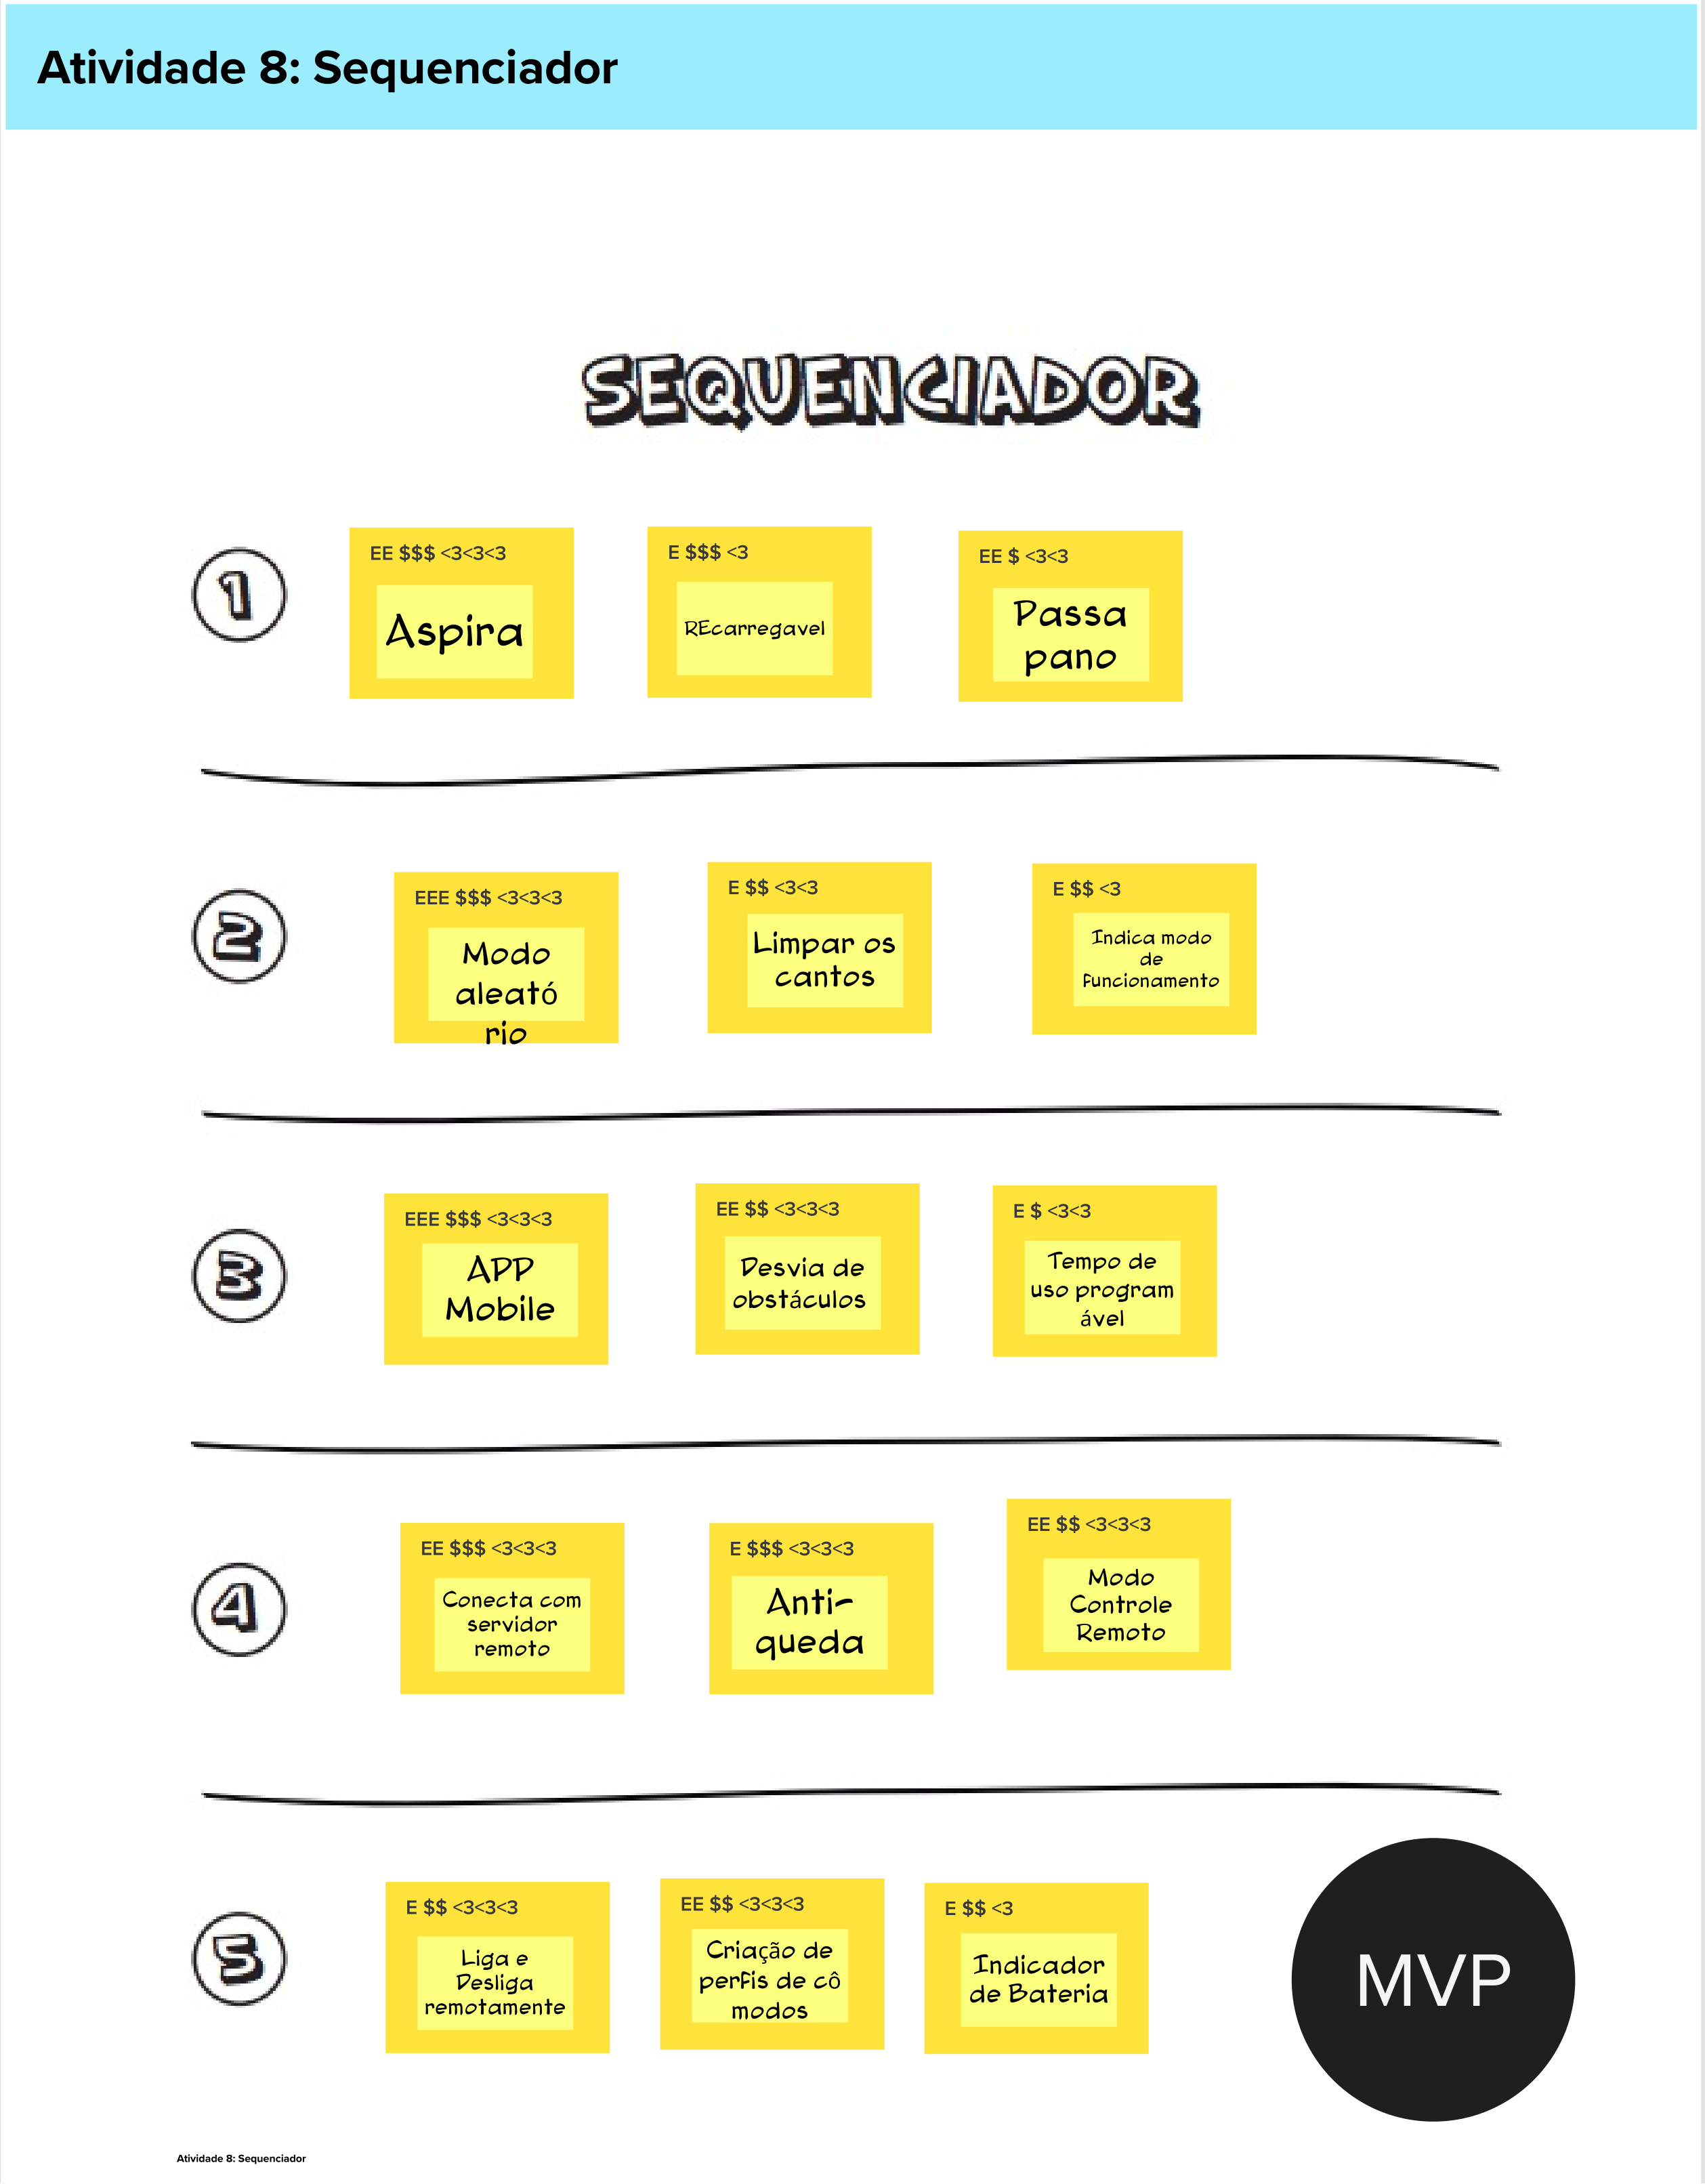
\includegraphics[height=0.7\textheight]{figuras/Lean Inception/Mural - Sequenciador.png}
\caption{Sequenciador de Funcionalidades \\ Fonte: Autoria própria, 2023.}
\label{sequenciador}
\end{figure}


\subsection{Premissas}
\begin{itemize}
\item O produto será utilizado exclusivamente para limpeza doméstica.
\item Deve ser utilizado apenas em ambientes fechados.
\item Será alimentado por bateria interna, mantendo sua autonomia pelo tempo mínimo pré-determinado. 
\end{itemize}

\chapter{Concepção e detalhamento da solução}
A seção 02 “Concepção e detalhamento da solução” se refere à fase 02 do ciclo de vida do projeto e tem por objetivo apresentar a arquitetura da solução/sistema para o problema.
\section{Requisitos gerais}
\label{requisitos}
	Para a elicitação dos requisitos do Quirby, a equipe utilizou, inicialmente, a técnica de brainstorm. Brainstorm é uma técnica desenvolvida em 1957 por Osborn e que promove a geração de um grande volume de ideias dentro de grupos. Estimulando a criatividade, um brainstorm permite que as ideias sejam compartilhadas sem a presença de críticas ao longo do processo (KING; SCHLICKSUPP, 2002, apud \cite{INOVAÇÃO}).
	Além do brainstorm, foi realizada uma Lean Inception entre os membros para contribuir com o levantamento de requisitos. Segundo Caroli (2018), as atividades realizadas durante o workshop proposto por esta técnica auxiliam no desenvolvimento de um produto de modo iterativo e incremental. 
	Por meio dessas técnicas, foram elicitados os requisitos funcionais e não funcionais do produto em desenvolvimento pela equipe. Estes estão dispostos nas Tabelas \ref{tab req} e \ref{tab req nf}. 

\begin{table}[H]
\centering
\caption{\label{tab req} Requisitos funcionais para o produto}
\begin{tabular}{|c|l|l|}
\hline
\rowcolor[HTML]{D9D9D9} 
\textbf{Requisito} & \multicolumn{1}{c|}{\cellcolor[HTML]{D9D9D9}\textbf{Descrição}}                                                                                                          & \multicolumn{1}{c|}{\cellcolor[HTML]{D9D9D9}\textbf{Observações}}                                                                                                                \\ \hline
\rowcolor[HTML]{DBEEF3} 
RF1                & \begin{tabular}[c]{@{}l@{}}O robô aspira o chão \\ do local posicionado.\end{tabular}                                                                                    &                                                                                                                                                                                  \\ \hline
\rowcolor[HTML]{DBEEF3} 
RF2                & \begin{tabular}[c]{@{}l@{}}O robô consegue limpar\\ os cantos da casa.\end{tabular}                                                                                      & \begin{tabular}[c]{@{}l@{}}Componentes giratórios com a capacidade\\  de chegar nos cantos, porém podem não ter\\  um desempenho completo de limpeza.\end{tabular}               \\ \hline
\rowcolor[HTML]{DBEEF3} 
RF3                & \begin{tabular}[c]{@{}l@{}}O robô é recarregado por \\ uma fonte de alimentação.\end{tabular}                                                                            & \begin{tabular}[c]{@{}l@{}} O Quirby é recarregado por meio\\ de uma fonte externa 12V, 1A. \end{tabular}                                                  \\ \hline
\rowcolor[HTML]{DBEEF3} 
RF4                & \begin{tabular}[c]{@{}l@{}}O robô tem um modo de \\ limpeza aleatória do local \\ posicionado.\end{tabular}                                                              &                                                                                                                                                                                  \\ \hline
\rowcolor[HTML]{DBEEF3} 
RF5                & \begin{tabular}[c]{@{}l@{}}Existe uma rotina do robô \\ que desvia de obstáculos.\end{tabular}                                                                           &                                                                                                                                                                                  \\ \hline
\rowcolor[HTML]{DBEEF3} 
RF6                & \begin{tabular}[c]{@{}l@{}}O robô consegue se conectar \\ a um ponto de acesso local pelo\\  protocolo de comunicação\\  IEEE 802.11\end{tabular}                        &                                                                                                                                                                                  \\ \hline
\rowcolor[HTML]{DBEEF3} 
RF7                & \begin{tabular}[c]{@{}l@{}}Um sistema deve espelhar seu\\  funcionamento e receber\\ operações em um aplicativo \\ Mobile.\end{tabular}                                  & \begin{tabular}[c]{@{}l@{}}A partir do aplicativo mobile, é possível\\ ter o relato do estado do robô, como \\ também processar funções de entrada \\ de operações.\end{tabular} \\ \hline
\rowcolor[HTML]{DBEEF3} 
RF8                & \begin{tabular}[c]{@{}l@{}}O robô relata ao usuário caso \\ tenha algum bloqueio em sua\\ movimentação que impede o \\ seu funcionamento padrão.\end{tabular}            &                                                                                                                                                                                  \\ \hline
\rowcolor[HTML]{DBEEF3} 
RF9               & \begin{tabular}[c]{@{}l@{}}Criação de protocolos de\\ comunicação entre o robô \\ e o servidor.\end{tabular}                                                             &  \begin{tabular}[c]{@{}l@{}}O Quiby deve se conectar a internet,\\ por meio de uma rede WI-fi 2.4GHz \\ e se comunicar com o servidor por\\ meio do protocolo HTTP.\end{tabular}                                                                                                                                                                               \\ \hline
\rowcolor[HTML]{DBEEF3} 
RF10               & \begin{tabular}[c]{@{}l@{}}Criação de protocolos de \\ comunicação entre o \\ aplicativo mobile e o \\ servidor.\end{tabular}                                            &                                                                                                                                                                                  \\ \hline
\rowcolor[HTML]{DBEEF3} 
RF11               & \begin{tabular}[c]{@{}l@{}}Desenvolvimento de um \\ banco de dados para \\ armazenar dados essenciais.\end{tabular}                                                      & \begin{tabular}[c]{@{}l@{}}Esses dados são relacionados ao login\\ de um usuário, e também suas operações,\\ logs de funcionamento, relatório de bugs.\end{tabular}              \\ \hline
\rowcolor[HTML]{DBEEF3} 
RF12               & \begin{tabular}[c]{@{}l@{}}O usuário consegue se \\ autenticar pelo aplicativo \\ mobile, tendo acesso às\\ funcionalidades do robô.\end{tabular}                        &                                                                                                                                                                                  \\ \hline
\rowcolor[HTML]{DBEEF3} 
RF13               & \begin{tabular}[c]{@{}l@{}}A partir do aplicativo Mobile,\\ é possível controlar os \\ movimentos direcionais do \\ robô através do protocolo\\  Bluetooth.\end{tabular} &                                                                                                                                                                                  \\ \hline
\end{tabular}
\end{table}

\begin{table}[]
\centering
\begin{tabular}{|c|l|l|}
\hline
\rowcolor[HTML]{D9D9D9} 
\hline
\rowcolor[HTML]{DBEEF3} 
RF15               & \begin{tabular}[c]{@{}l@{}}Através do aplicativo móvel, \\ é possível ligar e desligar o\\ robô de forma remota.\end{tabular}                                            &                                                                                                                                                                                  \\ \hline
\rowcolor[HTML]{DBEEF3} 
RF16               & \begin{tabular}[c]{@{}l@{}}É possível definir tempo de \\ uso operacional para ativar ou \\ desligar o sistema do robô.\end{tabular}                                     &                                                                                                                                                                                  \\ \hline
\rowcolor[HTML]{DBEEF3} 
RF17               & \begin{tabular}[c]{@{}l@{}}O robô consegue detectar \\ profundidade em seus passos\\ frontais, evitando então quedas.\end{tabular}                                       &                                                                                                                                                                                  \\ \hline
\rowcolor[HTML]{DBEEF3} 
RF18               & \begin{tabular}[c]{@{}l@{}}O robô indica a quantidade\\ de carga que a bateria armazena.\end{tabular}                                                                    &                                                                                                                                                                                  \\ \hline
\rowcolor[HTML]{DBEEF3} 
RF19               & \begin{tabular}[c]{@{}l@{}}O robô indica o modo de \\ operação que está trabalhando.\end{tabular}                                                                        & \begin{tabular}[c]{@{}l@{}}Essa indicação é tanto pela carcaça\\ do robô, quanto por um indicativo \\ digital, transmitida essa informação\\ pelo mesmo.\end{tabular}            \\ \hline
\rowcolor[HTML]{DBEEF3} 
RF20               & \begin{tabular}[c]{@{}l@{}}O robô deve conseguir ligar\\ e desligar por meio de comando\\ de voz pelo aplicativo da Alexa.\end{tabular}                                                                        & \begin{tabular}[c]{@{}l@{}}Deverá ser necessário a utilização do\\ aplicativo, Alexa para parear com o\\ Quirby.\end{tabular}            \\ \hline
\end{tabular}
\end{table}

\begin{table}[]
\centering
\caption{\label{tab req nf} Requisitos não funcionais para o produto}
\begin{tabular}{|c|l|}
\hline
\rowcolor[HTML]{D9D9D9} 
\textbf{Requisito} & \multicolumn{1}{c|}{\cellcolor[HTML]{D9D9D9}\textbf{Descrição}}                                                                                     \\ \hline
\rowcolor[HTML]{DBEEF3} 
RNF1               & \begin{tabular}[c]{@{}l@{}}O produto deve ter autonomia de,\\ no mínimo, 30 minutos.\end{tabular}                                                   \\ \hline
\rowcolor[HTML]{DBEEF3} 
RNF2               & \begin{tabular}[c]{@{}l@{}}A aplicação deve ficar disponível 24 horas, \\ 7 dias por semana para acesso pelo usuário.\end{tabular}                  \\ \hline
\rowcolor[HTML]{DBEEF3} 
RNF3               & \begin{tabular}[c]{@{}l@{}}O usuário deve conseguir utilizar o robô \\ mesmo sem acesso à internet.\end{tabular}                                    \\ \hline
\rowcolor[HTML]{DBEEF3} 
RNF4               & \begin{tabular}[c]{@{}l@{}}O sistema não apresentará aos usuários\\ quaisquer dados de cunho privativo.\end{tabular}                                \\ \hline
\rowcolor[HTML]{DBEEF3} 
RNF5               & \begin{tabular}[c]{@{}l@{}}O aplicativo deve funcionar em smartphones\\ com sistema Android 10 ou superior.\end{tabular}                             \\ \hline
\rowcolor[HTML]{DBEEF3} 
RNF6               & \begin{tabular}[c]{@{}l@{}}O Robô deve conseguir limpar cerca de 60\% \\ dos detritos de uma área de 2 m² em \\ 15 minutos de operação.\end{tabular} \\ \hline
\end{tabular}
\end{table}

 \section{Arquitetura Geral da Solução}
 Baseado na compreensão do problema e nos requisitos levantados para o produto, esta seção apresenta e detalha a arquitetura geral da solução a ser utilizada no projeto, envolvendo as diversas áreas de conhecimento.
 
\subsection{Arquitetura da Estrutura}
A arquitetura relativa à parte estrutural do projeto está apresentada na Figura \ref{arq estrut}.
Conforme o diagrama, percebe-se que o subsistema estrutural utilizará componentes embarcados, tais como: motores (de aspiração e deslocamento), mecanismos facilitadores de limpeza, sensores e outros componentes eletrônicos.
Inicialmente, para a estrutura externa do “Quirby”, pretende-se usar PLA (Ácido Polilático), por meio de impressão 3D.

\begin{figure}[h!]
\begin{center}
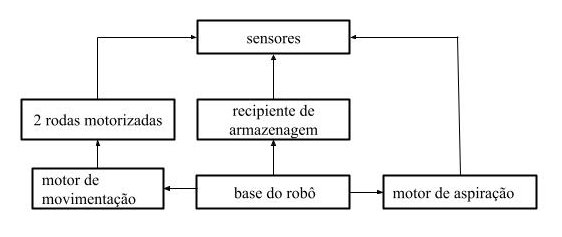
\includegraphics[width=\textwidth]{figuras/ar_estrut.png}
\caption{Arquitetura de Estrutura \\ Fonte: Autoria própria, 2023.}
\label{arq estrut}
\end{center}
\end{figure}

 O modelo deve conseguir agregar todos os componentes do robô, além de possuir dimensões que satisfaçam as condições de peso e locais de movimentação do “Quirby”, uma vez que o mesmo deve higienizar o chão embaixo de armários, cadeiras, etc.  
Constam nas Figuras \ref{fig2}, \ref{fig3} e \ref{fig4} um esboço primário da parte estrutural do projeto, ficando sujeito a alterações de design durante o decorrer da fabricação.
\\
\\
\\
\\  

\begin{figure}[h]
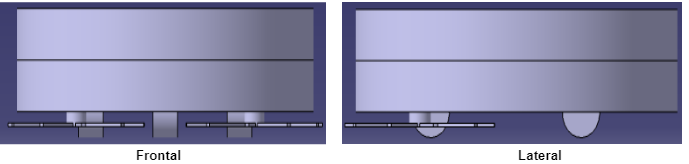
\includegraphics[width=\textwidth]{figuras/fig2.PNG}
\caption{Vistas Frontal e Lateral \\ Fonte: Autoria própria, 2023.}
\label{fig2}
\end{figure}

\begin{figure}[h]
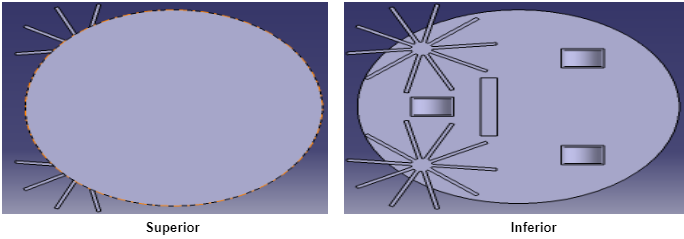
\includegraphics[width=\textwidth]{figuras/fig3.PNG}
\caption{Vistas Superior e Inferior \\ Fonte: Autoria própria, 2023.}
\label{fig3}
\end{figure}

\begin{figure}[h]
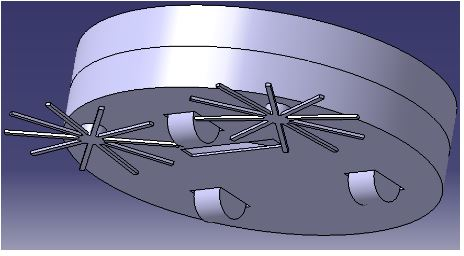
\includegraphics[width=0.5\textwidth]{figuras/fig4.jpg}
\caption{Vista Isométrica \\ Fonte: Autoria própria, 2023.}
\label{fig4}
\end{figure}


\subsubsection{Material}
O PLA (ácido polilático) é um termoplástico biodegradável de origem natural, obtido através de fontes renováveis. Material que detém elevada dureza, brilho e facilidade de impressão. Porém, apresenta algumas desvantagens, por exemplo, é um material de difícil fabricação e possui baixa resistência ao impacto. Foi escolhido para o projeto pela disponibilidade e por ser mais adequado à forma na qual o equipamento de impressão 3D disponível opera, que inviabiliza o uso de um outro material mais resistente.



\subsection{Arquitetura de Eletrônica}
A arquitetura para o subsistema de eletrônica utilizada foi o diagrama de blocos, como se observa na Figura \ref{fig6}. De maneira que a central poderá ligar e desligar, alterar modos de funcionamento, além de receber dados do robô como, por exemplo, porcentagem de bateria, o modo de funcionamento e a condição de bloqueio.
Também têm-se sensores para auxiliar o robô aspirador em sua movimentação desviando dos obstáculos; além da alimentação e a parte do acionamento dos diversos motores.

\begin{figure}[h!]
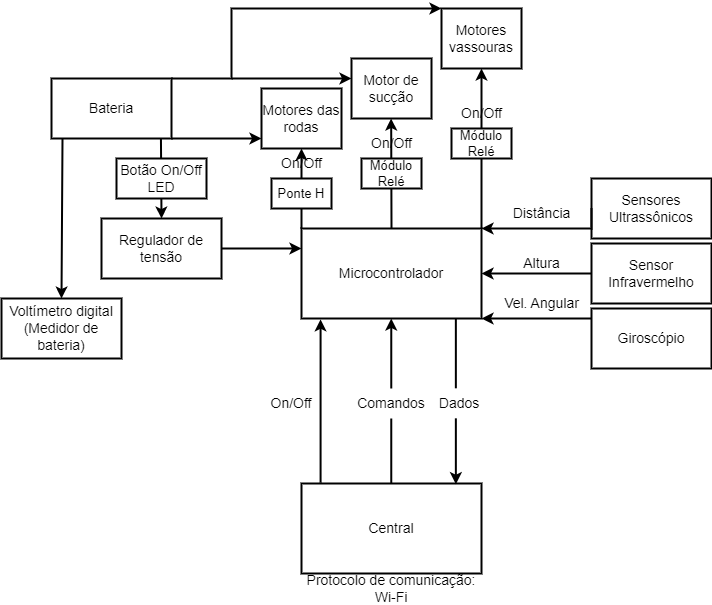
\includegraphics[width=\textwidth]{figuras/diagrama_bloco2.png}
\caption{Diagrama de Blocos \\ Fonte: Autoria própria, 2023.}
\label{fig6}
\end{figure}

\subsubsection{Definição de cada componente}
\begin{itemize}
\item \textbf{Central:} \\ É a parte do projeto responsável pelo controle e gerenciamento das trajetórias que o robô aspirador “Quirby” pode realizar. Será adotada uma central no projeto com o recurso de “Wi-Fi” para realizar a conexão do aplicativo com o protótipo do robô.
\item \textbf{Microcontrolador:} \\ É a parte do projeto responsável por executar as ações físicas, tais quais: controlar o movimento de trajetória do robô, controlar a rotação das vassouras e o acionamento do aspirador, além de realizar o processamento das informações recebidas pelos sensores. Será adotado o microcontrolador ESP32 \cite{ESPRESSIFMANUAL} para o projeto, pois este possui um excelente custo-benefício ao considerarmos as necessidades específicas do projeto “Quirby”, tamanho reduzido (auxilia na otimização do design), além de possuir módulo de Wi-Fi (recurso de suma importância para o presente projeto).
\item \textbf{Ponte H:} \\ Circuito responsável por fazer o controle de motores, como velocidade e sentido de rotação. No projeto será necessário o controle dos motores de sucção e de movimentação do robô, com isso a escolha da Ponte H se mostrou mais adequada para a implantação.
\item \textbf{Módulo Relé:} \\ Dispositivo responsável por fazer o chaveamento de cargas através de um sinal de microcontrolador. Para o projeto, será necessário o acionamento de dois motores DC usando o módulo relé.
\item \textbf{Motor de Sucção:} \\ É o componente responsável por realizar a principal função esperada para o projeto: aspirar. A maioria da poeira será removida por meio deste componente. Optamos por um motor 12 V e 2,5 A em conjunto com uma turbina, que já são utilizados em outras marcas de aspirador do mercado. 
\item\textbf{Motores das rodas:} \\ São os componentes responsáveis pelo deslocamento do robô, para que o mesmo possa realizar a limpeza em diferentes lugares.
\item\textbf{Motores das Vassouras:} \\ São componentes que consistem em motores rotativos ligados a uma caixa de redução para acréscimo de torque, que irão se manter ligados durante todo o funcionamento direcionando o pó e detritos para próximo do aspirador. Decidimos pelo modelo com 70 rpm por considerarmos que rotações mais altas poderiam espalhar mais detritos do que auxiliar o aspirador e 2,5 kg.cm de torque sendo mais que suficiente para não ser travado por obstáculos comuns. Chegamos nesses valores por possuírem características muito semelhantes com outros motores já utilizados no mercado de aspiradores robôs como, por exemplo, o CR120 DC3-12V \cite{aliexpress}.
\item \textbf{Sensores Ultrassônicos:} \\ Serão os componentes responsáveis por fornecer os sinais necessários para evitar o choque físico do robô contra objetos que podem o impedir de seguir sua trajetória. A maior aplicabilidade deste componente é para o uso do robô em modo randômico que, apesar de não possuir trajetória previamente definida, não causa colisões ou danos ao próprio robô ou demais objetos. Também serão aplicados no modo guiado, impedindo que o usuário, por distração, provoque uma colisão e, por consequência, um dano ao robô ou demais objetos.
\item\textbf{Sensor Infravermelho:} \\ É o componente que fica responsável por detectar se o robô irá cair de um degrau ou algo similar. O funcionamento será por meio de um sensor infravermelho na parte inferior do robô, desta forma, ao passo que não houver um chão ao nível adequado para o mesmo prosseguir com sua trajetória, o robô para de se deslocar, assim evitando sua queda e um possível dano irreversível aos seus componentes.
\item\textbf{Bateria:} \\ É o componente responsável por fornecer a energia para o funcionamento dos demais componentes ativos do projeto. Com o maior consumo energético do robô ficando por conta dos motores, principalmente o motor responsável por acionar a turbina que opera em 16 V e 1,5 A.

\begin{table}[H]
\caption{\label{tab 5} Componentes para confecção do Quirby}
\begin{tabular}{|c|c|c|c|c|}
\rowcolor[HTML]{D9D9D9} 
\textbf{Descrição}                                                                           & \textbf{Tensão}                              & \textbf{Corrente} & \textbf{Quantidade}                    & \textbf{Potência}                       \\
\rowcolor[HTML]{DBEEF3} 
\begin{tabular}[c]{@{}c@{}}Motor DC 6 V com caixa\\ de redução e Roda\end{tabular}           & 6 V                                          & 500 mA            & 2                                      & 6 W                                     \\
\rowcolor[HTML]{DBEEF3} 
\begin{tabular}[c]{@{}c@{}}Sensor Ultrassônico\\ Hc-sr04\end{tabular}                        & 5 V                                          & 15 mA             & 3                                      & 0,225 W                                 \\
\rowcolor[HTML]{DBEEF3} 
Esp32 Wifi Wroom-32                                                                          & 5 V                                          & 500 mA            & 1                                      & 2,5 W                                   \\
\rowcolor[HTML]{DBEEF3} 
\begin{tabular}[c]{@{}c@{}}Módulo Sensor de Reflexão \\ IR c/ Fotodiodo\end{tabular}         & 5 V                                          & 20 mA             & 3                                      & 0,1 W                                   \\
\rowcolor[HTML]{DBEEF3} 
\begin{tabular}[c]{@{}c@{}}Mini Motor DC N20 com Caixa \\ de Redução 6 V 70 RPM\end{tabular} & 6 V                                          & 50 mA             & 2                                      & 0,6 W                                   \\
\rowcolor[HTML]{DBEEF3} 
\begin{tabular}[c]{@{}c@{}}Conjunto Motor DC 12 V \\ Aspirador\end{tabular}                  & 16 V                                         & 1,5 A             & 1                                      & 24 W                                    \\
\rowcolor[HTML]{DBEEF3} 
Módulo Relê 5 V 10 A                                                                         & 5 V                                          & 20 mA             & 2                                      & 0,2 W                                   \\
\rowcolor[HTML]{DBEEF3} 
\begin{tabular}[c]{@{}c@{}}Mini Voltímetro Digital com \\ Amperímetro 10A\end{tabular}       & 5 V                                          & 15 mA             & 1                                      & 0,075 W                                 \\
\rowcolor[HTML]{DBEEF3} 
\hline
\multicolumn{1}{|l|}{\cellcolor[HTML]{DBEEF3}}         & \multicolumn{1}{l|}{\cellcolor[HTML]{DBEEF3}} & 3,260 A           & \cellcolor[HTML]{00FF00}\textbf{Total} & \cellcolor[HTML]{00FF00}\textbf{33,7 W}
\end{tabular}
\end{table}


Considerando a potência dissipada pelos principais componentes em total capacidade de uso, temos o valor aproximado de 33,7 W de potência dissipada e com uma corrente exigida das baterias de 3,260 A. Com esses valores, chegamos a conclusão de utilizar uma bateria com capacidade de 5000 mAh. Ela consegue fornecer 5 A por uma hora caso esteja totalmente carregada. Utilizaremos 4 baterias 26650 de 3,7 V em série para alcançar cerca de 14,7 V, tensão suficiente para alimentar todos os subsistemas do robô. 

\begin{table}[H]
\caption{\label{baterias} Baterias do Quirby}
\centering
\begin{tabular}{|c|c|c|c|}
\rowcolor[HTML]{D9D9D9} 
\textbf{Descrição}       & \textbf{Tensão} & \textbf{Corrente} & \textbf{Unidades} \\
\rowcolor[HTML]{DBEEF3} 
Liitokala Baterias 26650 & 3,7 V           & 5000 mAh          & 4                
\end{tabular}
\end{table}



\item\textbf{Botão On/Off:} \\ É um botão responsável por ligar ou desligar o robô.
\item\textbf{Regulador de Tensão:} \\ Dispositivo para manter a tensão dentro dos limites exigidos, para que o microcontrolador possa funcionar sem riscos. 
\item \textbf{Voltímetro Digital:} \\ O voltímetro é um instrumento para medir a tensão entre dois pontos \cite{dorf}, dessa forma há a possibilidade de observar a bateria e, através de seu display, permitir ao usuário a porcentagem da mesma.
\item\textbf{Sensor Giroscópio:} \\ Dispositivo para detectar velocidade angular nos 3 eixos. 
\end{itemize}

\subsection{Arquitetura de Software}
\begin{itemize}
    \item \textbf{Finalidade} \\ O documento de arquitetura de software tem como finalidade apresentar uma visão geral da arquitetura do projeto, evidenciando as decisões arquiteturais tomadas com intuito de informar aos desenvolvedores e stakeholders quais serão as tecnologias e a forma que elas serão utilizadas no produto, com intuito de evitar desentendimentos e contribuir com a consolidação um produto final sólido.
    \item \textbf{Escopo} \\ A intenção deste documento é captar os aspectos arquiteturais do sistema a ser desenvolvido para que ele atenda as necessidades do cliente final. Também é visado com este documento o entendimento de todos os membros da equipe de desenvolvimento, para evitar ruídos e falta de conhecimento de como deve-se desenvolver.
    \item \textbf{Visão Geral} \\ Será apresentada uma visão geral dos pontos iniciais a serem discutidos sobre a arquitetura do software, detalhando questões sobre como o sistema deve ser implementado e como ele deve se comportar. Será detalhada uma representação inicial da arquitetura tal qual como as metas e restrições dessa arquitetura.
    \item\textbf{Representação da Arquitetura} \\ A ideia para desenvolver o sistema do aspirador robô Quirby é utilizar-se do sistema de microsserviços, cujo objetivo é dividir a aplicação em blocos menores, evitando um sistema monolítico. Com isso, se tem facilidade na manutenção e na escalabilidade desse sistema, além de agilizar o desenvolvimento do mesmo \cite{supero_2020}.
\end{itemize}

Para desenvolvimento do aplicativo de celular do Quirby, foram definidos três microsserviços:

\textbf{1- Aplicação Mobile:} Parte que exigirá a autenticação do usuário, liberando então a visualização do estado de funcionalidade do Quirby. Também irá incluir criação de perfis e o controle do robô via bluetooth.

\textbf{2- Servidor Back-End:} Microsserviço responsável pelo gerenciamento do banco de dados, disponibilizando rotas para sua atualização. As seguintes tecnologias serão utilizadas para a construção deste serviço:

    \begin{itemize}
        \item Node JS
    
    O Node.js é uma plataforma construída sobre o motor JavaScript do Google Chrome (V8) para facilmente construir aplicações de rede rápidas e escaláveis \cite{nodejs_2019}. O Node.js usa um modelo de I/O direcionada a evento não bloqueante que o torna leve e eficiente, ideal para aplicações em tempo real com troca intensa de dados através de dispositivos distribuídos.
    
    Utilizamos o NodeJS como uma plataforma back-end que permite executarmos scripts Javascript no lado do servidor para acessar e trabalhar de maneira rápida, recebendo e enviando informações utilizando o protocolo HTTP com pacotes no formato JSON para comunicação. O fato de não possuir dependências facilita o processo de desenvolvimento, deploy e integração contínua do código.
    
    Considerando o tempo disponível para a conclusão da aplicação, o NodeJS atendeu todas a nossas demandas, economizando o tempo de aprendizado que seria necessário com outras linguagens como, por exemplo, PHP ou RUBY.
    
    A forma com que o NodeJS gerencia os requests por um looping de eventos permite que a aplicação trabalhe em paralelo e de forma assíncrona, suprindo a demanda da aplicação de agilidade para execução das ações. Com o IO não-bloqueante oferecido pelo NodeJs, as tarefas do aplicativo do Quirby podem ser executadas em background e o retorno de sucesso ou falha dessas tarefas ocorre através de uma função de callback.
    
    \item PostgresSQL
    
    PostgreSQL é um sistema de gerenciamento de banco de dados de código aberto altamente escalável e robusto \cite{POSTGRESSQL}. Ele suporta diversos tipos de dados, incluindo estruturados, semi-estruturados e não estruturados, e possui recursos avançados como transações, gatilhos, armazenamento de objetos e indexação. 
    
    \begin{comment}
    \begin{figure}[h]
        \centering
        
\includegraphics[scale=0.6]{figuras/postgres.png}
        \caption{Postgres\cite{POSTGRESSQL}}
        \label{postgres}
    \end{figure}
    \end{comment}
    
    O PostgreSQL é amplamente utilizado em aplicações de missão crítica e é compatível com a maioria das plataformas de desenvolvimento de software. Ele é amplamente utilizado por organizações de todos os tamanhos, desde pequenas startups até grandes corporações. 
    
    Nesta aplicação este SGBD será utilizado para armazenar as informações dos usuários do sistema e do robô Quirby. Decidimos por sua utilização baseados na familiaridade da equipe com a tecnologia e por ser suportado através de um sistema de contâineres pelo Heroku, nosso servidor em ambiente de produção.
    
    \item Sequelize
    
    O Sequelize é um ORM (Object-Relational Mapping) que se utiliza de uma técnica de programação que permite que os desenvolvedores trabalhem com dados relacionais utilizando objetos em vez de usar código SQL diretamente \cite{sequelize_2022}. Isso significa que os desenvolvedores podem trabalhar com os dados de um banco de dados utilizando as mesmas estruturas de dados e os mesmos métodos que utilizam para trabalhar com outros objetos em sua aplicação. Esta possibilidade contribui para a legibilidade e manutenibilidade do código, além de ajudar a isolar a lógica de banco de dados da lógica de negócios. 
    
    O Sequelize foi utilizado em nosso back-end para a geração das tabelas Pessoa e Robô no banco de dados e para a realização de consultas de maneira mais rápida e simples.
    
    \item Google OAuth API
    
    A API de autenticação do Google é uma plataforma baseada em nuvem que possibilita a autenticação em sistemas por meio de contas do Google \cite{google_2022}. Dentro da nossa aplicação, esta API permite que os usuários entrem em suas contas do Google para acessar o Quirby App, sem precisar criar uma nova conta. O Google OAuth oferece suporte a vários fluxos de autenticação, incluindo o fluxo de autenticação implícito, o fluxo de autenticação de código e o fluxo de autenticação de senha, como apresentado na Figura \ref{googleAuth}.
    
    Além destes fluxos, o Google OAuth também permite que nosso sistema obtenha informações públicas do perfil do usuário, como o endereço de e-mail e o nome, com o intuito de personalizar a experiência do usuário no Quirby App.
    
    \begin{figure}[h]
        \centering
        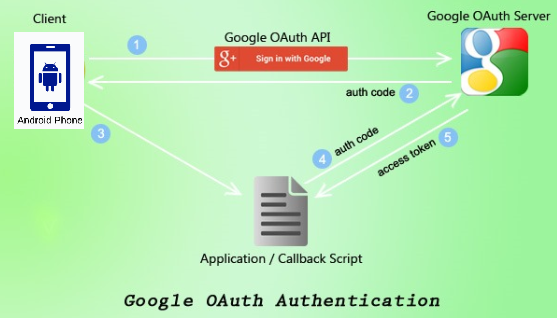
\includegraphics[scale=0.6]{figuras/googleAuth.png}
        \caption{Funcionamento da API do Google API \\ Fonte: Modificado de \cite{PHPPOT}}
        \label{googleAuth}
    \end{figure}
    
    \item Alexa
    
    Alexa é uma assistente virtual desenvolvida pela Amazon. Ela é capaz de responder perguntas, controlar dispositivos domésticos inteligentes, reproduzir música e fornecer informações através de comandos de voz. A Alexa é acionada por um comando de ativação, geralmente "Alexa" e depois pode ser usada para realizar várias tarefas, como reproduzir música, fornecer notícias e previsão do tempo, controlar dispositivos da smart home, entre outras funções \cite{amazon}. 
    
    \begin{figure}[h]
        \centering
        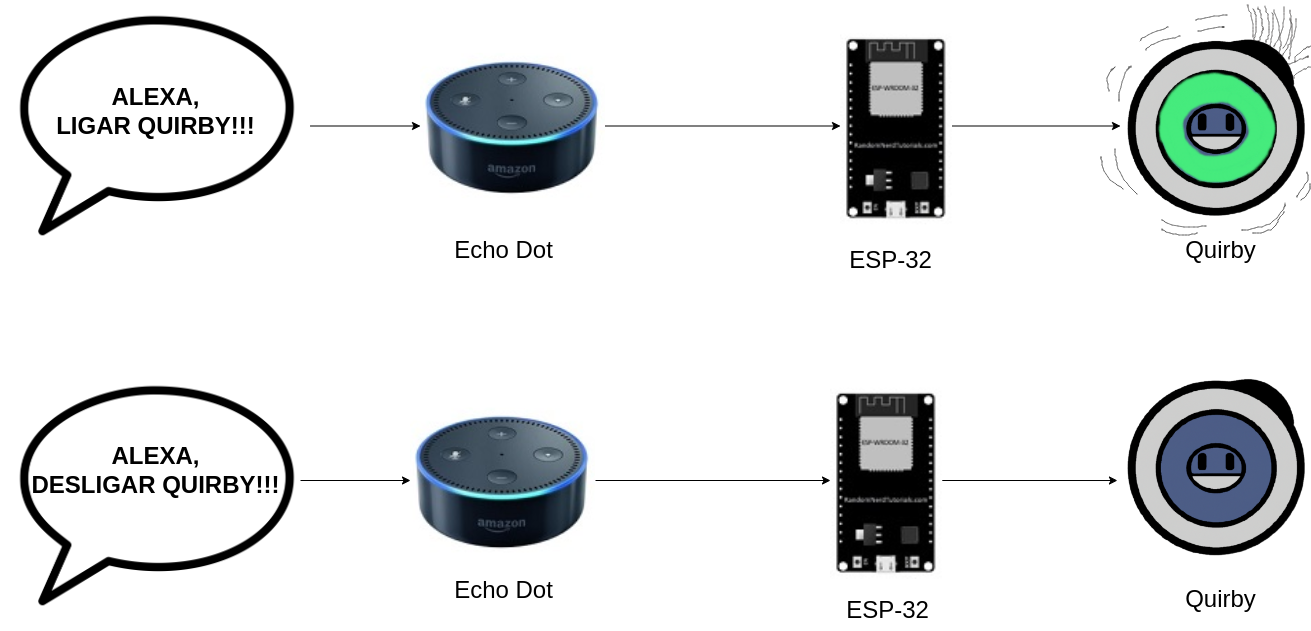
\includegraphics[scale=0.3]{figuras/alexaQuirby.png}
        \caption{Exemplo de utilização do Quirby com a Alexa \\ Fonte: Autoria própria, 2023.}
        \label{alexaQuirby}
    \end{figure}
    
    A Alexa também pode ser integrada com outros serviços e aplicativos para expandir suas funcionalidades, como o uso de skills (habilidades) desenvolvidas por terceiros. A Alexa está disponível em dispositivos como o Amazon Echo, Echo Dot, Echo Show, entre outros. 
    O seu ecossistema será utilizado para Ligar e Desligar o Quirby atráves de comandos de voz em qualquer lugar do mundo, como apresentado na Figura \ref{alexaQuirby}.
    \end{itemize}

\textbf{3- Sistema Embarcado:} Microsserviço responsável pela solução computacional do Quirby, com a implementação de um sistema de tempo real. Tendo no sistema embarcado a execução de tarefas em real-time, orientado a deadlines, com o uso otimizado de memória. Irá então receber e tratar as informações recolhidas pelos sensores, sendo que após essa tarefa de aquisição, o sistema irá realizar tarefas que envolvem o funcionamento da parte de limpeza do robô. Também irá se comunicar pelo protocolo IEEE 802.11, mandando e recebendo informações da situação no servidor na nuvem. Terá a disponibilidade de se comunicar via Bluetooth para realizar as interrupções que acarretam ao movimento a partir da aplicação mobile.

A relação entre os três microsserviços listados estão expressos na Figura \ref{arquiteturaGeral}.\\
\begin{figure}[h!]
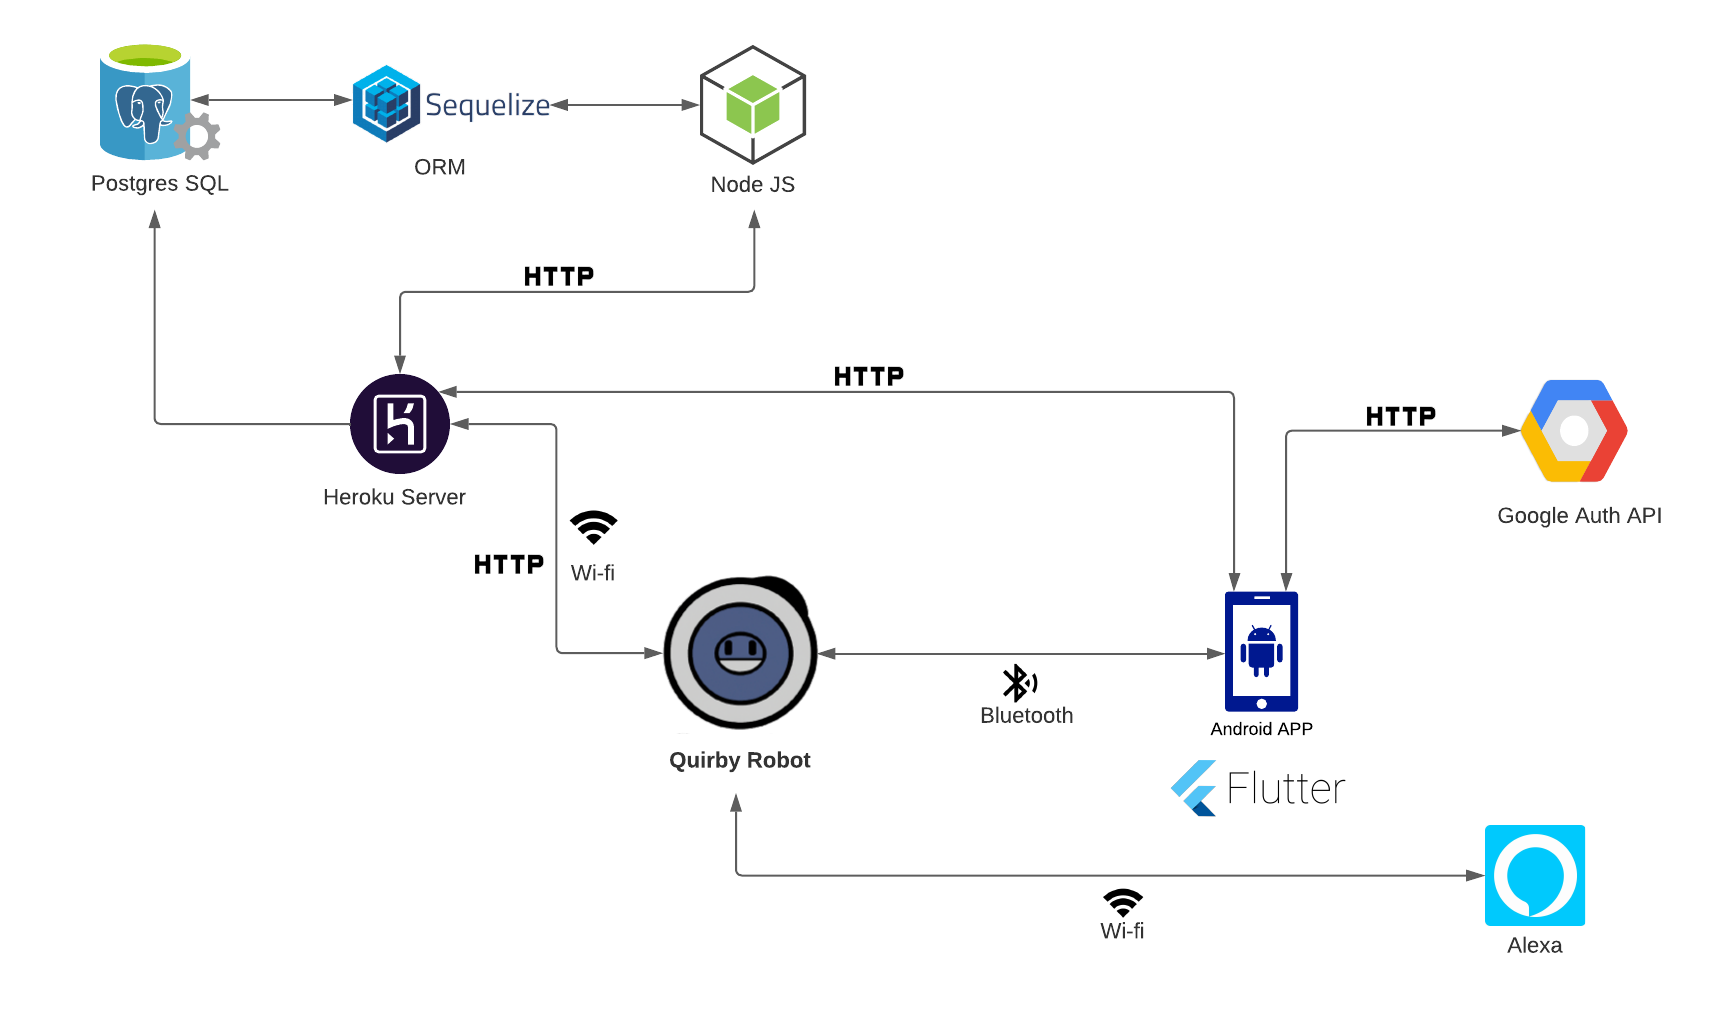
\includegraphics[width=\textwidth]{figuras/software/arquiteturaQuirby.png}
\caption{Arquitetura Geral do Sistema \\ Fonte: Autoria própria, 2023}
\label{arquiteturaGeral}
\end{figure}

\begin{itemize}
\item \textbf{Metas e Restrições de Arquitetura}\\
\textbf{Metas}:\\
\quad Funcionar em celulares com sistema operacional Android.\\
\quad Conexão remota via aplicativo ao Quirby.\\
\quad Conexão via bluetooth para controle direcional do Quirby.\\
\\
\textbf{Restrições}:\\
\quad Conexão a internet.\\
\quad Conexão com a API.\\
\quad Conexão com o banco de dados.\\
\end{itemize}

\subsection{Arquitetura de Integração}
Para representar a Arquitetura de Integração de todos os subsistemas, foi escolhido o diagrama de blocos, visando demonstrar sucintamente a integração existente entre as partes do sistema. Na Figura \ref{fig8}, é possível identificar que o sistema eletrônico será acoplado à estrutura do Quirby, encaixando suas partes de forma que facilite a movimentação do robô. Além disso, o sistema de software será integrado ao sistema eletrônico, por protocolos de comunicação adequados para um sistema embarcado, fazendo com que seja possível  a comunicação remota entre o robô e o aplicativo mobile.

\begin{figure}[h!]
    \centering
    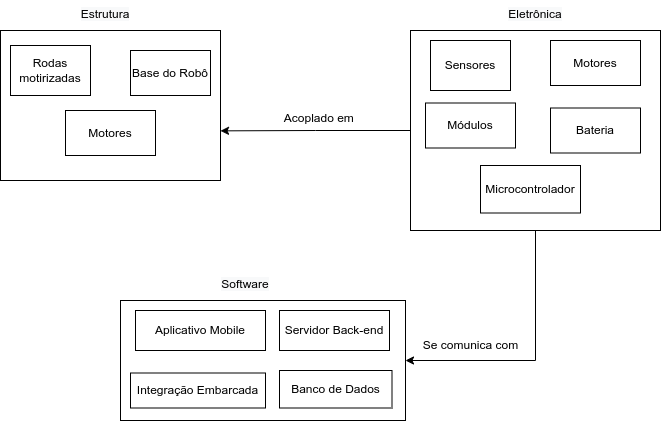
\includegraphics[width=15cm]{figuras/Diagrama sem nome.drawio.png}
    \caption{Arquitetura de Integração \\ Fonte: Autoria própria, 2023}
    \label{fig8}
\end{figure}